\clearpage

\section{Orthonormalization}

\begin{refsection}

\begin{tcolorbox}	
	\begin{tabular}{p{2.75cm} p{0.2cm} p{10.5cm}} 	
		\textbf{Header File}   &:& orthonormalization.h \\
		\textbf{Source File}   &:& orthonormalization.cpp \\
        \textbf{Version}       &:& 20190225 (Daniel Pereira)\\
	\end{tabular}
\end{tcolorbox}

This block applies a Gram-Schmidt orthonormalization procedure to the input signal.

\subsection*{Input Parameters}

This block has no input parameters.

\subsection*{Methods}

Orthonormalization(initializer\_list$<$Signal *$>$ \&InputSig, initializer\_list$<$Signal *$>$ \&OutputSig) :Block(InputSig, OutputSig)\{\};
\bigbreak
void initialize(void);
\bigbreak
bool runBlock(void);

\subsection*{Functional description}

This block orthonormalizes the data by implementing a Gram-Schmidt algorithm~\cite{arfken99}. This is implementation follows the topology presented in Figure~\ref{fig:orthonormalizationDiagram}.
%
\begin{figure}[h]
\centering
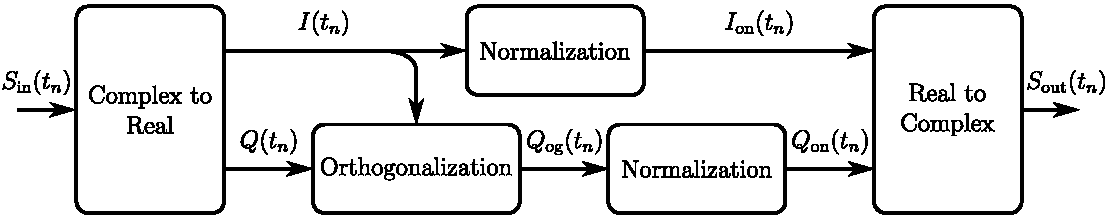
\includegraphics[width=\linewidth]{./lib/orthonormalization/figures/diagramDSP_GS}
\caption{Block diagram representation of the Gram-Schmidt orthonormalization procedure.}
\label{fig:orthonormalizationDiagram}
\end{figure}
%
The input signal $S_\text{in}(t_n)$ is separated into its in-phase and in-quadrature components, $I(t_n)$ and $Q(t_n)$, the amplitude of the in-phase component, $P_I$, is estimated as the average of its square, ie.:
\begin{equation}
P_I=\text{mean}(I^2(t_n)),
\end{equation}
the in-phase signal is then normalized, ie.:
\begin{equation}
I_\text{on}(t_n)=\frac{I(t_n)}{\sqrt{P_I}}.
\end{equation}
The in-quadrature component is then orthogonalized in relation to the in-phase component
\begin{equation}
Q_\text{og}(t_n)=Q(t_n)-\frac{I(t_n)\text{mean}(I(t_n)Q(t_n))}{P_I},
\end{equation}
which is then normalized in a manner similar to what was done for the in-phase component
\begin{align}
P_Q=\text{mean}(Q_\text{og}^2(t_n)),\\
Q_\text{on}(t_n)=\frac{Q_\text{og}(t_n)}{\sqrt{P_Q}}.
\end{align}
Finally, the two orthonormalized components are combined to form the output signal
\begin{equation}
S_\text{out}(t_n)=I_\text{on}(t_n)+iQ_\text{on}(t_n)
\end{equation}

\subsection*{Input Signals}

\textbf{Number:} 1
\textbf{Type:} Complex signal

\subsection*{Output Signals}

\textbf{Number:} 1\\
\textbf{Type:} Complex signal

\subsection*{Sugestions for future improvement}

\begin{itemize}
	\item Add the optimized recursive Gram-Schmidt algorithm as an option.
\end{itemize}

% bibliographic references for the section ----------------------------
\clearpage
\printbibliography[heading=subbibliography]
\end{refsection}
\addcontentsline{toc}{subsection}{Bibliography}
\cleardoublepage
% ---------------------------------------------------------------------



%\bibliography{./lib/photoelectron_generator/photoelectron_generator}